% !TEX TS-program = pdflatex
% !TEX encoding = UTF-8 Unicode

% This is a simple template for a LaTeX document using the "article" class.
% See "book", "report", "letter" for other types of document.

\documentclass[11pt]{report} % use larger type; default would be 10pt

\renewcommand{\chaptername}{} % reports say "Chapter"... don't!

\usepackage[utf8]{inputenc} % set input encoding (not needed with XeLaTeX)
\usepackage{float}
\usepackage{gensymb}

%%% Examples of Article customizations
% These packages are optional, depending whether you want the features they provide.
% See the LaTeX Companion or other references for full information.

%%% PAGE DIMENSIONS
\usepackage{geometry} % to change the page dimensions
\geometry{a4paper} % or letterpaper (US) or a5paper or....
% \geometry{margin=2in} % for example, change the margins to 2 inches all round
% \geometry{landscape} % set up the page for landscape
%   read geometry.pdf for detailed page layout information

\usepackage{graphicx} % support the \includegraphics command and options

% \usepackage[parfill]{parskip} % Activate to begin paragraphs with an empty line rather than an indent

%%% PACKAGES
\usepackage{booktabs} % for much better looking tables
\usepackage{array} % for better arrays (eg matrices) in maths
\usepackage{paralist} % very flexible & customisable lists (eg. enumerate/itemize, etc.)
\usepackage{verbatim} % adds environment for commenting out blocks of text & for better verbatim
\usepackage{subfig} % make it possible to include more than one captioned figure/table in a single float
% These packages are all incorporated in the memoir class to one degree or another...

%%% HEADERS & FOOTERS
\usepackage{fancyhdr} % This should be set AFTER setting up the page geometry
\pagestyle{fancy} % options: empty , plain , fancy
\renewcommand{\headrulewidth}{0pt} % customise the layout...
\lhead{}\chead{}\rhead{}
\lfoot{}\cfoot{\thepage}\rfoot{}

%%% SECTION TITLE APPEARANCE
\usepackage{sectsty}
\allsectionsfont{\sffamily\mdseries\upshape} % (See the fntguide.pdf for font help)
% (This matches ConTeXt defaults)

%%% ToC (table of contents) APPEARANCE
\usepackage[nottoc,notlof,notlot]{tocbibind} % Put the bibliography in the ToC
\usepackage[titles,subfigure]{tocloft} % Alter the style of the Table of Contents
\renewcommand{\cftsecfont}{\rmfamily\mdseries\upshape}
\renewcommand{\cftsecpagefont}{\rmfamily\mdseries\upshape} % No bold!

%%% END Article customizations

%%% The "real" document content comes below...

\title{Just-In-Time 3D Printing}
\author{Theodore Boyd, Lucy Campbell, James Hennessey}
\date{} % Activate to display a given date or no date (if empty),
         % otherwise the current date is printed 

\begin{document}
\maketitle

\chapter{Executive Summary}
In this report we discuss the research, development and analysis of our VEIV EngD group project. The focus of this work is on the field of 3D printing, specifically looking at improving the printing experience through near to real-time error mitigation.

The first part of this report covers the wider set of ideas behind our work on how that 3D printing errors can be lessened through allowing the user to manipulate the print whilst it it taking place. We then look at the structure of our task and its progress, followed by a study of the current state of the art and a look at possible approaches in the Prior Art chapter. Here we also analyse the current 3D printing approach and pipeline which we will need to build upon.

Next, we detail our approaches to the proposed solutions in the Method section, specifically looking at the programming and surveying techniques and their respective implementations and results. This is followed by a case study based investigation of that work in our Evaluation chapter, showing what we can do that previously was not possible.
Finally, we look forward to future developments and applications opened up because of our project in Future Work, and any concluding remarks and lessons learnt in the Conclusion section.

In summary, we have found, through our combined efforts, that with this upcoming new technology of 3D printing, there are a broad range of uses and applications. As the user base widens, so increases the noticeability of the failings and drawbacks of 3D printing. There are numerous annoyances with the process that we detail and tackle, including warping of prints, extrusion failures and long preparation times.

We detail relevant research, submit questionnaires to learn from experts and amateur users alike and write a software improvement to implement a new feature to help mitigate that particular problem.

At the end, we analyse the overall 3D print workflow and the features we have added along the pipeline, evaluating whether and how much we have improved the situation, through time saving or otherwise. We conclude that while 3D printing is still a fairly error-prone process, we have added substantially new features to the software that make the task more convenient.


\tableofcontents


\chapter{Introduction}
\section{Project Proposal}
The objective of this project was to advance the state-of-the-art of 3D printing. In particular the goal was to find ways to interact with and control a 3D printer `just-in-time'. Just-in-time refers to being able to control the commands sent to the printer just before they are about to be interpreted and executed by the printer. The just-in-time period is not fixed as the printer is continuously printing the object, building it up layer upon layer as is typical in all additive manufacturing. The kinds of interaction and control remained open to be influenced by the discoveries of the group as the project evolved and new discoveries were made.

The group explored the impact that just-in-time control might have on the diverse applications of 3D printing technology. The group has engaged in a dialogue with 3D print users and investigated the context within which 3D printing is emerging. 

The key principle that guided the software development process was to harness the existing software design patterns in the already open-sourced software, trying to work at a higher-level of abstractions, rather than low-level code. For example we wanted to avoid working on the firmware on the 3D printer. For a short period, we did explore the printer's firmware, to discover how feasible programming it might be and found it to be somewhat opaque and obtuse. Whilst raw access to the printer could have been useful, we deemed direct physical motor control and serial communication management as outside the scope of our project.

A second guiding principle of the project was that the software developed should remain open-source. ``Open-source is an approach to design, development, and distribution offering practical accessibility to a product's source''~\ref{reference:1}. This approach was partly taken because the 3D printers used in the project are built using open-source hardware (OSH) and operated using open-source software (OSS). The software used in the project was Cura, which is particular to the Ultimaker 3D print machines --- also used throughout. Cura and Ultimaker are one set of open-source 3D print technologies, existing alongside for example ReplicatorG software which controls, amongst other printers, the Makerbot range, all of which act upon Arduino microcontroller boards (pieces of open-source hardware found at the source of many open-source hardware devices today)~\ref{reference:1}. 

The final guiding principle in our project was to focus more heavily on expert users by not developing novice user interfaces. This decision was made slightly after the start of the project, in light of the initial gains made in the software development process leading to a more detailed understanding of the kind of control and interaction possible. 

Interviews and surveys were conducted in order to establish the wider context of the project's stakeholder groups in a landscape of existing 3D print technology capabilities, the needs of expert print users as well as some novice users, potential applications and relevant contemporary academic research.  

There were many unknown elements as to how far the group might be able to develop the just-in-time capabilities of a 3D printer. Ideas began broad and included a host of possible avenues for both applications and software development, gradually becoming more focused and specialised as the project unfolded, continuously guided by the overarching principles outlined above. The group maintained an exploratory approach throughout, creating stage deliverables as the project unfolded. 




\section{Project Structure}
We were a self-managed group, with internally negotiated roles and planning development decided through weekly meetings. Further monthly meetings were held with our academic supervisor Prof. Anthony Steed, to reflect upon progress and to discuss next steps.  In accordance with the recommendations of the academic supervisor the group maintained an online record of all group project materials using Google Groups and Google Docs. 

The project was chosen by the group from a number of others presented by academic staff and students to the entire VEIV 2014 class on the 6\textsuperscript{th} of November. Anthony Steed set forth the idea as a way for a group to explore 3D printing and potential for real-time haptic control. The group, who had already formed by this stage chose Anthony's idea largely to pursue a shared interest in 3D printing and as an opportunity to diversify from their thesis topics. 

The group member responsibilities were:
\begin{itemize}
\item Project management: Lucy
\item Software Development: James
\item Software Development: Theo
\end{itemize}

The project time frame was nine months. The project deliverables were set in collaboration with our supervisor and evolved alongside our understanding of both the software and 3D printing as a phenomena. The project timeline was as follows, starting in 2013 ending in 2014:

\begin{itemize}
\item Late October the group first formed. 
\item Early November projects suggestions were discussed and the idea chosen 
\item November 26\textsuperscript{th} progress report with Anthony 
\item December 27\textsuperscript{th} internal group presentation of summary of progress 
\item January 7\textsuperscript{th} next steps set forth and agreed by group.
\item February 4 \textsuperscript{th} group presented informally to the rest of VEIV cohort 
\item June 20\textsuperscript{th} first draft of report 
\item July 1\textsuperscript{st} project presented to the exam board
\item July 4\textsuperscript{th} project report submission deadline 
\item First week after Easter final report and presentation (may be presented before a public audience)
\item Regular weekly meetings were held throughout. 
\end{itemize}

The requirements of this project are therefore set to ensure group members come from across more than one academic department. In this project for example members came from schools of architecture and computer science, with expertise ranging for example from front end software development to machine learning to mathematics to service and estates management. 

This VEIV project is an interdisciplinary project~\ref{reference:4},~\ref{reference:7}. As is often the case with software development groups in the commercial world and knowledge working practices this group was a one off formation~\ref{reference:9}. The VEIV school has facilitated the project in a number of ways: first enabling access to academic expertise and leadership in the form of a project supervisor, secondly providing desk space to work together as a group, thirdly giving access to resources such as 3D printers and print materials, fourthly by allocating time in our academic schedules to produce the project and finally there will be structured criticism and feedback to prepare individuals in the group for similar future experiences. The project acted as an opportunity to reflect upon how best to bring together and work within groups of people with disparate academic experience in one off situations and produce tangible outcomes, a subject of current focus in UCL and the wider academic community~\ref{reference:5},~\ref{reference:6},~\ref{reference:8},~\ref{reference:10}. 

The associated academic faculties of this project, from which resources were provided via the VEIV program structure, were Computer Science (where the VEIV school staff and students reside in large part), the Make Space which is a cross departmental workshop space providing materials and equipment such as 3D printers as well as technical support, and finally the Bartlett faculty of the Built Environment who supported our project to a smaller extent, providing secondary academic support and meeting spaces (also where a further cohort of the VEIV school reside).

The support that is mentioned above was effective in facilitating team working in the project, in particular the group found that having physical space to work together facilitated understanding of new concepts presented by members in light of their different academic backgrounds. The academic leadership gave the group focus, greater access to physical resources which was essential in progressing our work. The structural guidelines set forth by the VEIV school were also invaluable. Ours was a small group, formed prior to choosing a project to work on, we felt that these were positive factors in the project, giving us greater cohesion and control of the project. 

We openly shared ideas within the group as well as with the wider 3D print community, communicating on online forums and through surveys. Our group embraced the structure of the VEIV project as an opportunity to collaborate openly and work in a team, to increase the accessibility and generalisability of our work using broader methods and more accessible language to record and communicate our work~\ref{reference:5},~\ref{reference:6}. 

We chose to work on OSS as the machines that we used operate on OSS. The group sought guidance about Cura from within the existing code itself and via online discussion forums. There is little formal documentation and guidance about the development of Cura, a common, well-accepted challenge when developing OSS~\ref{reference:11}~\ref{reference:60}. Using OSS was an opportunity to make a direct contribution to a community of developers who will hopefully build upon the innovations of just-in-time control~\ref{reference:12},~\ref{reference:67}. 





\section{Motivation}
Our group was delighted to have an opportunity to work in such an active field of research. 3D printing is a phenomenon that captures widespread attention at many levels of society around the world, it is the source of much anticipated opportunity for economic success and has generated a seemingly exponentially growing industry~\ref{reference:13}. Associated research about 3D printing has been complimentarily intense and the potential applications are wide ranging and continuously evolving~\ref{reference:17}. 

One of the overarching ideologies emerging from the barrage of developments in 3D printing is that manufacturing and product development are now increasingly happening from the bottom up, with individuals able to print any object within their price range and within the receding limitations of the technology available from home~\ref{reference:13}. It has been speculated that 3D printing will change the integral nature of manufacturing along with the associated logistical and production processes involved, as people gain the ability to manufacture at the at the user's location~\ref{reference:16}. Anxiety has arisen over the accessibility of 3D printing and its potential applications, fuelled by media stories for example about 3D printed guns~\ref{reference:15}. Regulation, design patents and copyrights on 3D printed objects may therefore have an increasing impact~\ref{reference:13}. While the regulatory aspects of 3D printing may seem unrelated currently, such matters may be a growing consideration in any resultant applications of our project. To name an example, if a design was patented and our new system then reproduced an altered that design, would it belong to us or to the original designer?

Although the potential of 3D printing is vast, there remains much research and development work still to be done to improve the quality of the technologies and software available, to make them more accessible to a wider set of users and capable of creating more complex objects. There are persistent limitations to 3D print technologies, for example the ``stair-stepping'' effect of fused deposition model (FDM) technologies, explained in more detail in Section \ref{section:TechnologyLandscape} of the report, whereby ``parts cannot accurately conform to the CAD geometry in the vertical plane''~\ref{reference:18}. This was reported in~\ref{reference:44} and was reiterated last year by Nannan and Ming in their paper on Additive manufacturing: technology, applications and research needs~\ref{reference:17},~\ref{reference:18}.

3D printing processes are unreliable across the spectrum of the different kinds of technologies available for different reasons. While failure rate increases in the lower costing 3D print machines such as the Ultimaker and RepRap, failures become more costly in higher end commercial machines where occurrences are fewer, however waste more time and potentially finite and costly materials as well as causing wear and tear to the machines themselves. Given the widespread and impeding level of errors encountered in 3D printing technologies, this was a most compelling motivation for our project and a central objective of our group was to apply just-in-time control of a 3D printer to solve recurring errors. 

One cross section of 3D print users who we were particularly interested in and who commonly use the same machines available to us throughout our project can loosely be described as the `maker' community. While the trend of making is broader than 3D printing alone, groups are utilising the technology and incorporate open software and hardware technologies such as Arduino and Cura in their work. ``The availability of low-cost machines allowed other projects to start, inspired the `makers' movement, helped the diffusion of fablabs and prototyping boards such as the Arduino, and it even started an economy''~\ref{reference:19}. Some examples of maker community groups who utilise similar technologies to us are the HackSpace or Makerverse who are resident in London or attendees of the MakerFair conference events, who are strongly linked to academic research and institutions as well~\ref{reference:14}. We feel that these groups share our project ethos of exploring accessible technologies for people to use to aid innovation. 

As our group work uses similar technology and has a similar outlook as the maker community our project has an inherent strong link to the creative and generate innovative applications being explored. It was therefore natural that we consider how the just-in-time capabilities that we developed might also benefit the lineage of designers and artists using 3D printing.  

Even though we are motivated by the types of work happening in maker communities, by contemporary research and by applications in design, the problem of errors occurring in the 3D printing process is overarching and much of our work has been informed by contemporary academic research, discussed in the section of this report entitled Current Approaches, as well as by discussions with commercial 3D print users. We were unable in the given timeframe to address all potential applications of `just-in-time' control, for example commercial application of our project as a design tool would require a more robust investigation of user interfaces, and there are a plethora of industries actively researching 3D printing such as aerospace, transport or fashion not discussed here.





\chapter{Prior Art}
\section{Technology Landscape}
\label{section:TechnologyLandscape}
While our project used an Ultimaker FDM printer, there are a number of ways to produce a three-dimensional physical object using machinery. They usually fall into either additive or subtractive techniques. Before the advent of modern technologies, additive techniques were based around pouring materials into moulds and subtractive techniques used tools such as chisels and lathes to sculpt larger blocks of raw material into the final output~\ref{reference:23}.

In recent decades, we have seen a new innovation in the form of three-dimensional object production using automation and information technology (IT). Automation involves both mechanisation and industrialisation of techniques, while the use of IT allows for computerised systems to pre-program parameters, batch processing jobs and ease repetitive or high-volume tasks.

New technologies have opened up new subtractive forms. They include for example computer numerical control (CNC) mills and routers. The additive form is that associated with the field of 3D printing~\ref{reference:20}. 

Additive manufacturing (AM) is today synonymous with 3D printing\footnote{However, in the literature, the terms did not traditionally cover the same fields.} and it has become an ever more popular and useful technique with a growing number of applications and a shrinking of price points~\ref{reference:27}. AM can take a number of forms~\ref{reference:23} but is broadly defined as a collection of computer-controlled processes of creating parts in a layerwise fashion, that is joining of a layer of material onto layers laid down or cured previously, without part-specific tooling~\ref{reference:34}. A reference definition is provided by the American Society for Testing and Materials (~\ref{reference:59}, ASTM) as ASTM F2792–10. Subtractive forms of manufacture are more traditional and there is general agreement amongst those using the technology, that additive forms can work with increased accuracy, precision and resolution~\ref{reference:26}.

Availability of 3D computer models was crucial to realising the concept of layered object creation, but other technologies such as affordable laser systems, photocurable materials, and powerful personal computers helped to disseminate this technology as well~\ref{reference:24}. Critical enabling developments included the advent of desktop computers and the economic development and availability of industrial lasers~\ref{reference:25}.

Forms of AM include the use of heated extrusion of materials (especially thermoplastics but also rubber) known as fused deposition modelling (FDM). FDM is particularly popular due to the relatively low cost of materials and high commercial potential easing its spread into the non-professional market from AM's origins as a professional tool. We shall cover FDM in more detail later as it is the format our printer used. The printer we have chosen is the Ultimaker --- low specification machines such as the Ultimaker can retail at under £1,000~\ref{reference:28} and previous models such as the Reprap have even been specifically designed to be self replicating, inherently widening their accessibility, see Figure~\ref{figure:FDM}.

\begin{figure}[H]
  \centering
  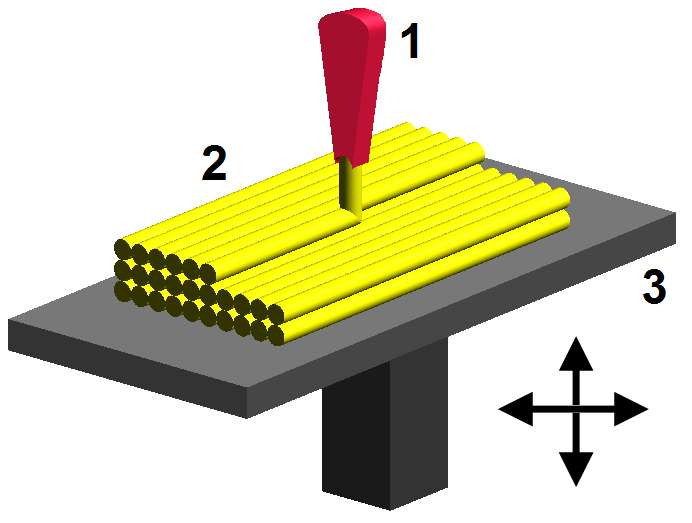
\includegraphics[width=4in]{FDM_by_Zureks.png}
  \caption{Fused deposition modelling schematic~\ref{reference:35}}
  \label{figure:FDM}
\end{figure}

Other AM processes use beams of electrons or photons (lasers) to create pools of molten metals, known as Electron Beam Freeform Fabrication (EBF3) or if not melting it completely, sintering. For powdered metals and other granular materials, there is also a similar process called Direct Metal Laser Sintering (DMLS) and its variants~\ref{reference:29}.

For more challenging materials than metals and plastics, more complex techniques have been developed. For plaster, binder can be printed onto the particles using an inkjet head (similar to those used in standard 2D printing) to selectively bind particles from a larger powder bed~\ref{reference:30}. For paper and films made of plastics and metals, Laminated Object Manufacturing (LOM) uses a laser beam to cut out the current layer's shape before the film rollers roll out a new layer on top to cut~\ref{reference:31}.

It is also possible to use light sensitive chemicals for an approach that allows for construction not constrained by the printer rig's dimensions. Known as photopolymerisation or stereolithography, this approach solidifies, or cures, a light-sensitive material such as a gel or liquid, by applying light beams to locations in a bath of the material that are to be part of the object, leaving the remainder uncured and reusable. Through the raising or lowering of the laser or bath, layers can be constructed in a similar fashion to more standard, dry methods of additive manufacturing. A variant, Mask Projection Stereolithography (MPS) machine projects a light beam mask over the material bath surface to protect the material that does not need to be cured~\ref{reference:33}, see Figure~\ref{figure:SLA}.

\begin{figure}[H]
  \centering
  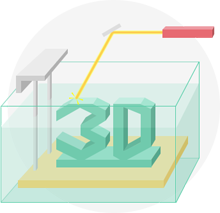
\includegraphics[width=3in]{sla.png}
  \caption{Photopolymerisation~\ref{reference:32}}
  \label{figure:SLA}
\end{figure}

With the recent consumerisation of fused deposition modelling, this method of 3D printing has received a large amount of coverage and usage in recent years. It is an important area of growth with a very broad range of uses, reaching into art and design as well as manufacturing, construction and prototyping. Initially only a professional's tool, FDM and AM as a whole is now accessible to many hobbyists, proving its worth in society as a hacker's or maker's tool mentioned previously, drawing many similarities to the initial growth of the personal computer market at the end of the last millennium~\ref{reference:21},~\ref{reference:22}.

A widening audience has also brought to light a number of problems with the nascent technology. And so we have found now to be the opportune time to experiment with, and attempt to solve, a number of these as it is of utmost importance that this technology grow and be further explored to perhaps give it the chance that the personal computer was given previously.

Whilst all of additive manufacturing is very applicable today, FDM in particular is a very promising new technology for wide distribution, and so it would be particularly beneficial to the fabrication community as a whole to address the most frequent hurdles encountered in it. It also gives us the chance to focus our efforts on one of the more popular modes of AM, reaching the widest popular audience whilst still being able to produce targeted solutions that are not too diluted by abstraction to the variants of AM.




\section{Current Approaches}
\label{section:CurrentApproaches}
This section discusses work being done in recent years, that shares common characteristics with our project. Much of the work discussed is focused on prototyping processes, ranging from rapid tooling engineering to medical prototyping~\ref{reference:42},~\ref{reference:44}. 

There are a number of projects which analyse 3D models before printing them, to calculate the correct geometries of a shape for some particular set of optimisations and alter it accordingly through a series of algorithmic equations. The project Make It Stand: Balancing Shapes for 3D Fabrication made it possible to interactively deform an existing model, pre-empting print failures by altering the mesh of the model. Researchers addressed the problem of how to balance a 3D model, as often a printed object would be weighted incorrectly because of overhangs and the centre of mass makes it unbalanced~\ref{reference:36}. The project applies an algorithm to manually carve and deform a model using the initial surface mesh as an input and relaying back to the user who manually alters the model until it is optimally positioned, sized and weighted to `stand up'. 

The project, Making Burr Puzzles from 3D Models optimises and arranges the orientation of a model in the pre-processing phase, splitting complex 3D shapes into puzzle pieces automatically~\ref{reference:43}. Others have updated the model to strengthen the object being printed, redistributing mass where points are particularly thin for example~\ref{reference:45}. Such projects achieve structural analysis on the user side which, with conventional tools is often infeasible as it requires specialised training and software. ``Trial-and-error, the most common approach, is time-consuming and expensive''~\ref{reference:46}. 

In Selective laser sintering (SLS) printing techniques there is active research into how the level of errors incurred can be mitigated, although Tang et al. argue more generally that it is impossible to achieve perfection in AM techniques~\ref{reference:37}. One of the central drives for improving outcomes, in part comes from the potential to use SLS processes in medical research, for example to fabricate prototypes from biomedical images in maxillofacial surgery procedures~\ref{reference:38},~\ref{reference:39}. Research papers focusing on this particular application analyse the accuracy and reliability of SLS processes~\ref{reference:38},~\ref{reference:39}, however the solutions offered are limited, finding errors through trial and error or improving upon this by calculating for errors in the pre-processing phase, similar to the examples mentioned above. This inherently means that the user must know the potential errors and or abort the print job once it has begun. This is particularly wasteful in scenarios when the print time extends over several hours, after which the user returns to find the failed print, wasting materials and time. 

Current related projects work at the pre-processing phase in comparison to our project which deals with the manufacture stage, although they do focus on foreseeing and mitigating errors. 

In the context of work being done to improve reliability of different industrial manufacturing processes, there has been some breakthrough in automating feedback about the object once manufacture has begun, using sensors and an understanding of different kinds of shape optimisation. Improvements to the machinery itself and reliability of materials are often a central focus in contrast to the examples above, which focus heavily on areas of high level programming~\ref{reference:37}. In research by Shin et al. into Layered Manufacturing (also referred to as Solid Freeform Fabrication), they introduce feedback loops to the manufacture process in the form of sensors and a camera, in order to alter an object as it is being produced.

\begin{figure}[H]
  \centering
  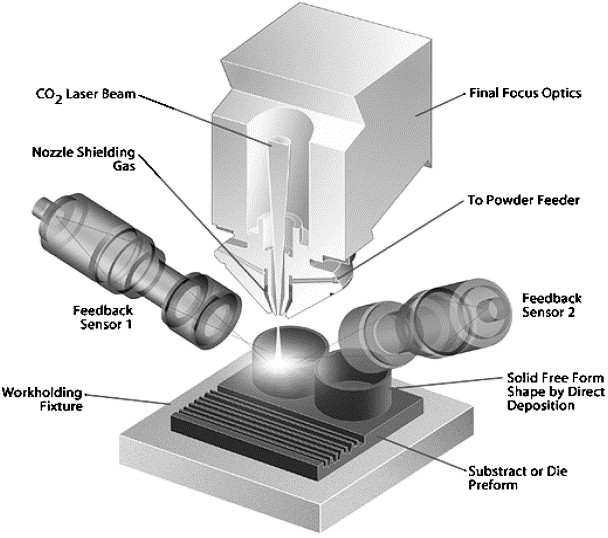
\includegraphics[width=4in]{shin.jpg}
  \caption{Direct metal deposition layered manufacturing system~\ref{reference:40}}
  \label{figure:Shin}
\end{figure}

The image in Figure~\ref{figure:Shin} shows that based on the material properties of the object the optimal density can be calculated in relation to specific stress points while the manufacture is taking place, to make changes in the materials during the print process~\ref{reference:40},~\ref{reference:41}. The process of change happens as the material is being extruded. The developments made by the research groups above brings the alteration process into the manufacture phase in a similar way to our project and further is able to incorporate information about the already printed parts of the object.  

In sum, rapid prototyping is becoming more or less standard in product development and a second wave of technological creativity is finding its way to industrial practise. The approaches mentioned above are set apart from our research as we are exploring new interesting areas, after the printing process has already begun coupled with more widely available low-cost FDM print technology. 




\section{Pre-Existing Pipeline}
\label{section:PreExistingPipeline}
The pre-existing pipeline for fused deposition modelling (FDM) 3D printers involves a number of steps, firstly a 3D model is prepared for printing, then the 3D model is `sliced' into commands that a 3D printer can execute, thirdly these commands are sent to the firmware running on the 3D printer and finally the 3D printer interprets and executes said commands. These four stages of the pipeline will be outlined in detail below. 

\textbf{Preparing a 3D model}: Once a 3D parametric model is ready to be printed it can be loaded into a software application to prepare it further. The application used throughout the project is Cura --- an open source-application created by Ultimaker, although there are other applications that function in a similar way.

Once the model has been loaded into Cura the user has the option to specify a number of settings for the print. The most important of these are:

\begin{itemize}
\item Fill density of the model
\item Thickness of the solid top / bottom layers
\item Printhead speed
\item Type of structural supports
\item Type of platform adhesion
\item Thickness of plastic
\item Size and position of skirt
\item Nozzle temperature
\end{itemize}

These settings control both how the model should be printed, how dense it should be and also how the printer should print it, how fast should it try and go. Both have significant impact on how the object will be printed and need to be specifically chosen for the model being printed. For example, a very intricate model would benefit from being printed at a slower speed. Similarly, if the printer has only just been turned on it is much more likely to require more time to heat up, to ensure that the printer is extruding correctly without blockages.

Once these settings have been chosen, the model can be `sliced' into g-code with these parameters included.

\textbf{Slicing}: In Cura the slicing process is done by a separate piece of software, hidden from the user called the CuraEngine. It takes a parametric model, potentially from a number of file formats (slt, obj, ply), along with print settings as input. Then it finds the best way to represent the model using a sequence for one dimensional commands that the printer can execute, known as g-code, to outline the shape and fill the inside of the model with an appropriate structure, illustrated below:

\begin{figure}[H]
  \centering
  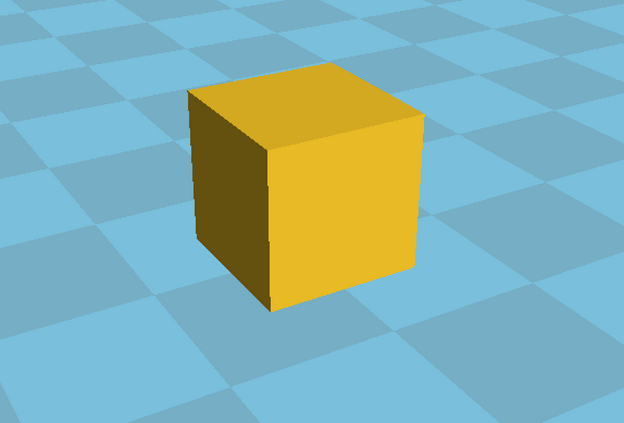
\includegraphics[width=4in]{james_cura_top_fig.png}
  \caption{Parametric representation of a cube, within Cura.}
  \label{figure:JCtop}
\end{figure}

\begin{figure}[H]
  \centering
  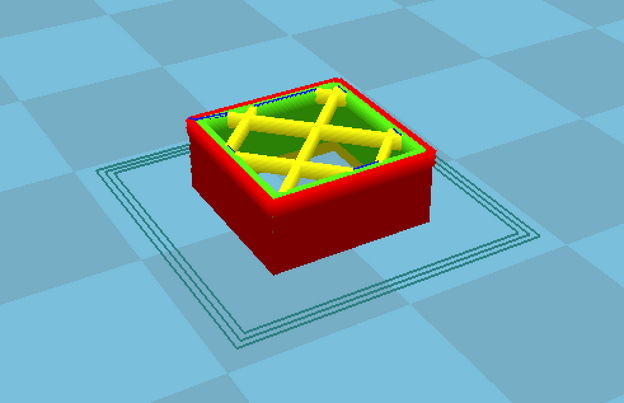
\includegraphics[width=4in]{james_cura_bottom_fig.png}
  \caption{Commands comprising cube in previous figure.}
  \label{figure:JCbottom}
\end{figure}

Figure~\ref{figure:JCtop} is a parametric representation of a cube. The second is a rendered version of the g-code generated from slicing the model. Each layer is made up of individual g-code commands, which represent a single line of plastic. Each of these lines are printed one at a time then once a layer is completed the printer moves along the z axis, before printing the next layer. The inner fill of the cube follows a crosshatch pattern for stability in this example, covering 20\% of the inner density (which would have been specified by the user).This image also shows the skirt, which is the outer square on the first layer of the print, designed to ensure that the printer is extruding correctly before starting to print the cube itself.

In addition to movement commands shown in Figure~\ref{figure:JCbottom} the g-code also includes commands to control the temperature of the nozzle, fan speed and extrusion motor. A more detailed description of individual g-code commands will follow later.

\textbf{Communicating with the printer}: The two methods for transferring the g-code to the printer are to either use an SD card inserted directly into the printer or to communicate over a USB cable connected to the computer, however both are very similar.

Once a connection between the printer and the computer is established (the SD card is built on an Arduino so it is also a computer), the firmware will make a request for more information. The computer will then send as many lines of g-code as it can, until the buffer on the firmware is full and no more can be received. As commands are continuously executed and the buffer empties, the firmware requests more gcode. In this model the g-code is sent to the printer in arbitrarily large blocks with no recognisable relation between the groups of commands contained within. Thus once a model has been sliced and the g-code has begun to be sent to the printer, it cannot be changed as there is no way to determine what has or has not been sent already.

The only deviation from the above model is that occasionally the firmware will make a request to resend a line of code. The computer will resend this line, then continue sending sequentially from this line onwards. 

Interpreting and executing the g-code: The firmware has a buffer of g-code commands that it takes individually, interprets and executes using the various motors and controls on the printer. 

For example the following six lines of g-code are interpreted to perform the following actions:
\begin{verbatim}
G1 F2400 E0.00000
G1 F1200 X111.50 Y93.50 E0.33859
G1 X111.50 Y111.50 E0.67718
G1 X93.50 Y111.50 E1.01577
G1 X93.50 Y93.50 E1.35436
G0 F9000 X98.10 Y93.50 Z0.40
\end{verbatim}

Which equates to the following script:\\
\\
Set the printers relative extrusion amount to zero\\
Move in a straight line from its current position to a new coordinate (111.50, 93.50) on the Cartesian plane while extruding from the previous E value, E0.0,  to E0.3.\\
Move in a straight line to (111.50, 111.50) while extruding to E0.67\\
Move in a straight line to (93.50, 111.50) while extruding to E1.01\\
Move in a straight line to (93.50, 93.50) while extruding to E1.35\\
Keep the X and Y axis fixed and move along the Z axis to 0.4 while not extruding\\

If you look at this g-code in detail you can see that is is drawing a square on one layer before moving vertically, at which time it would continue to print the next layer. The insight from this example is that g-code can easily be split into layers when there is a movement along the Z axis. Furthermore the E value needs to always remain relative to the previous value. 




\chapter{Method}
\label{section:Method}
\section{Surveys}
In order to understand our target users better and to develop aims in line with the wider 3D print community we conducted an initial online survey to establish what the main problems of 3D printing were and asked for a more detailed forecast on what users might use our technology for. 

While the initial survey was targeted at the maker community and research groups directly surrounding us, we also later engaged with commercial 3D print companies and retailers to find out more about what kinds of problems they faced and whether their experience was a shared one, which we found was the case. In the second survey we sent an email to commercial users. 

Participants in the initial survey represent a number of different fields; predominantly architecture, fine art, computer science, teaching, biology and engineering. Many of the respondents mentioned that they use 3D printing for fun alongside their academic work. 

From the list of possible drawbacks regarding which errors were most frequently encountered, print failures and print times were listed most often and by the most diverse range of survey participants. This was a central theme in the later survey as well.

Certain user groups were more interested in improving specific functionality. Colour restrictions were a concern for survey participants based in the arts, as well as for those using the technology to create gifts. If we were to have focused more heavily on improving the colour restriction we might have spoken in more depth to these groups as well as having worked more closely with 3D printers that have multi-colour functionality. 

Strength of material was a concern for those working in areas related to rapid prototyping and creating commercial prints however effected artists as well. Certain issues were commonly shared such as the drawbacks of cost of materials, although as the cost of the type of material being used increases the nature of cost concerns ties into more complex issues of business profits and decisions on retail price. For those printing for personal use, the cost issue is only about how to fund the materials. 

The list in Table~\ref{table:Surveys} is of some survey participants predictions for what they can imagine doing with a 3D printer if it could edit a model in real time, some general themes arose from answers, centred around using the technology for encouraging experimentation in the design and creative process, customisation of objects and correcting print failures.


\begin{table}[h]{\begin{minipage}{\textwidth}
\begin{tabular}{| p{2cm} | p{12cm} |}
\hline
\textbf{Profession} & \textbf{Response} \\\hline

EngD Researcher & I'd try out new ways of interpreting data in physical forms using real time information.\\\hline
Research Engineer & Just experimenting with a fun interface.\\\hline
Teaching fellow & I'm not quite sure how that would work, but I could imagine that I would be a lot more experimental in my designs. Usually my designs are very much fixed by the time it comes to the print stage, so any afterthoughts or adjustments get left and/or forgotten about.\\\hline
Academic & Cope with print failures.\\\hline
Sculptor & Developing intricate abstract forms. versatile scale changes to object, on the fly modifications saving proofing time.\\\hline
Architect & Not much that can't be done without that technology. I suppose it could automate mass-customization of products, so a person didn't need to make the customizations to the file manually.\\\hline
Architect & Not sure about that. I cannot see how the design outcome can be controlled. Maybe to fix flaws in geometry?\\\hline
Architect & Using it as a sketch tool to develop and demonstrate different ideas.\\\hline

\end{tabular}
\caption{Survey responses to ``What could you imagine doing with a 3D printer if it could edit a model in real time?''.}
\label{table:Surveys}
\end{minipage} }
\end{table}

On reflection of the first survey a larger survey population including a more diverse range of users was found to have been desirable. We incorporated the initial responses from academic and maker communities into the early brainstorming and investigation phases of the project and went on to conduct more open ended surveys with expert 3D print users operating commercially and selling print bureau services.. The second survey was conducted further into the project duration and was aimed at developing our understanding of the kinds of errors that may be incurred. The kinds of industries using the professional 3D printing services on offer range from educational bodies, hobbyists to architects' offices, large scale manufacturers and medical manufacturers, to corporations searching for novel project delivery methods. The associated processes of commercial printing are more costly and time consuming than those in the initial survey. 

Similarities arose amongst both groups, methods of fixing errors in extrusion based printers are similar in machines across different price ranges available. For example the founder of a prominent research group in London's 3D printing community, offering commercial advice and workshops reported back that he runs 4 machines 6 days a week 24 hours. ``I usually experience 2/3 errors during prints per week, we have a lot of control over the most minor of parameters within the bundled software, this however means tweaking the machine before each print which is a hassle!'' [Section~\ref{section:AppendixA}]. Our group conducted similar manual fixings using the Ultimaker. 

It is similarly necessary to control the speed of FDM printers manually to suit the print job being carried out. Using just-in-time control would allow for this to occur as the print is being carried out, to slow down during more complex sections and speed up  over simple shapes. 
 
The surveys were aimed at a broad spectrum of 3D print users and not only restricted to understanding users of one type of printer. Problematic printing processes were felt as strongly by those talking about the lower end FDM printers utilised in this project, as well as those using 3D printers associated with commercial processes. 

At the more expensive end of the spectrum, for example SLS machines were reported to be problematic as dust gathers in the powder to cause errors, and higher end FDM printers also experience the same nozzle blockages as the lower grade machines used in our project. Other common problems included misaligned objects, long and inaccurate print time estimation that meant users come back to find failed prints. For a full list of the feedback given please see the Appendix, Section~\ref{section:AppendixA}.






\section{Buffer Control}
\label{section:BufferControl}
\begin{figure}[H]
  \centering
  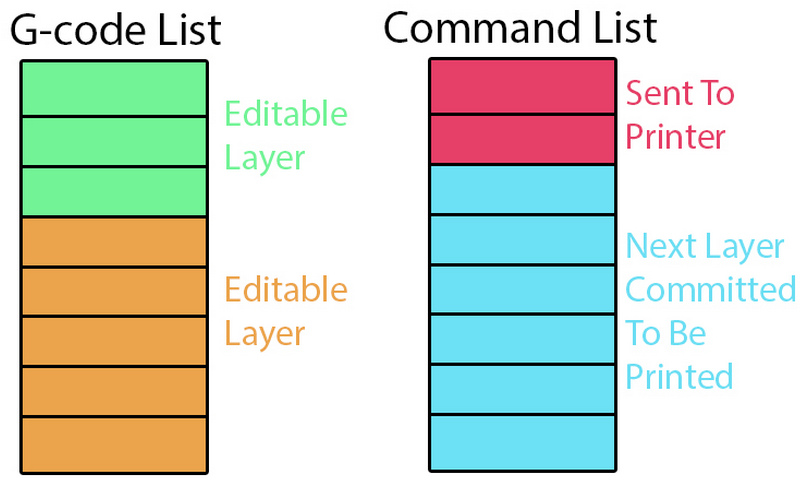
\includegraphics[width=4in]{james_two_lists.png}
  \caption{Our new list-based buffer system.}
  \label{figure:Jlists}
\end{figure}
In this section we discuss our software development. In Section~\ref{section:PreExistingPipeline} of this report we outlined how the g-code, generated by the slicer, is sent to the printer in arbitrarily large chunks. If we wanted to enable just-in-time control of the printer we needed to create a pipeline that controls what g-code and when it is sent over the serial port to the firmware. We achieved this by introducing a new buffer on the computer's side of the serial port.

To implement this new buffer on the computer's side we needed to introduce a number of different data structures as well as adapting existing ones. Originally Cura kept all of the g-code in an array with a pointer to the next command being sent; a simple but effective system. We kept this implementation, however rather than adding all g-code into this array (now known as the command list) at once, groups of g-code are added a layer at a time and only when the queue of commands remaining is very small (we found 6 remaining commands to be a good threshold). Keeping this implementation also allowed for the firmware requests to resend a line, described in Section~\ref{section:PreExistingPipeline}, to be unaffected. We can now think of this command list as the g-code commands that are committed to being printed --- meaning that they cannot be altered and are going to be sent to the firmware next.

In addition we introduced a second array known as the g-code list, it contains the remaining g-code commands produced by the slicer. When a new layer needs to be added to the command list, it is taken from this g-code list and appended to the back of the command list. The g-code list can be thought of as a staging area, where the commands can be edited, then removed so new ones can be added.

Having introduce our new buffer system the challenge now was to find a way to enable this layer-based control. With knowing how many commands are in each layer and subsequently how many commands should be taken from the g-code list to the command list. Fortunately, when the g-code is returned from the slicer it includes meta-information designed to assist in the rendering of the g-code. This includes comments where a new layer is being started. Below is an example from a real file:
\begin{verbatim}
;LAYER:1
M106 S127
G0 F9000 X98.10 Y106.90 Z0.40
;TYPE:WALL-INNER
G1 F1620 X98.10 Y98.10 E8.73536
G1 X106.90 Y98.10 E8.79054
\end{verbatim}

Using meta-information, such as \verb|;LAYER:1|,  we could build a cumulative histogram representing the number of lines in each layer. We could then use this no know how many g-code commands to release into the command list. 

These small additions to the pipeline have the advantage of knowing what has already been committed to be printed and allows for the g-code not yet committed to be changed using different methods, the applications of which will be discussed in subsequent sections. However, next we will discuss what this layer-based control enabled us to do in the context of working with pure g-code. 

One of the parameters FDM 3D printers have is the thickness of the plastic that is extruded from the nozzle. It is this thickness --- a constant for a whole model --- that determines the height of each layer. With this insight it makes it possible to switch the g-code list for any other g-code list and cumulative layer histogram that uses the same thickness of plastic. All that is required for seamless switching is to keep a pointer to the cumulative histogram of the layer that is to be sent next. When the g-code is switched, the pointer to the next command from the g-code list to be added to the command list is updated by taking the value from the new cumulative histogram. So when the command list has fewer than 6 commands in, the next layer added will be at the perfect height from the last layer printed. 

This generic method for switching g-code can be used in a number of different applications, which are discussed later. An important thing to remember at this stage is that this process is completely agnostic to what the g-code commands are. It is possible to replace the g-code list with a completely random g-code that will execute in mid air causing a print failure. As such, the onus is on the applications that generate new g-code, ensuring that the next layer is aligned with the previous.





\section{G-code Manipulation}
\label{section:GCodeManipulation}
Once we replaced the original buffer system used by Cura with our own, we could manipulate individual commands sent to the printer and therefore gained more direct control over when the printer performed certain actions.

We had to take into account a small delay over the serial cable connection (via USB) to the printer, approximates to about one standard g-code instruction. With this in mind we are able to change the pending instruction just-in-time, before being sent to the printer and executed in its modified form.

Our initial explorations of g-code manipulation involved learning what the often cryptic instruction lines meant. We studied the codes manual for the predecessor of our printer called the RepRap as it shares most, if not all of the same codes with our printer~\ref{reference:47}. Since g-codes are a standardised system originally written for CNC mills and similar equipment, some of the terms are fairly generic and sometimes their meaning is misused when applied to 3D printing. For example, whilst G0 (rapid movement) and G1 (controlled movement) have different meanings for a CNC equipment, they are identical when interpreted by the Ultimaker. Also, codes such as M240 (start conveyor belt motor) have no meaning at all in our scenario.

Looking at the codes applicable to 3D printing, we noted that most of them are in the form of:
\begin{verbatim}
<CODE>
\end{verbatim}
or
\begin{verbatim}
<CODE> <PARAMETERS>
\end{verbatim}

Where \verb|<CODE>| is a placeholder for g-code such as G0 or G1 that instructs the printer and \verb|<PARAMETERS>| is a list of preset options that clarify those instructions. For example, these could be the X and Y coordinates to which the G1 instructs the printer head to move. Some parameters are optional in the \verb|<PARAMETERS>| list as well. For example, the Z coordinate and extrusion amount (symbolised by the letter E) are not necessary for G1 to execute.

Once we had learnt the relevant codes and what their parameters meant, we could begin to deconstruct incoming commands in our buffer, manipulating, reconstructing and sending them off to the printer. This process involved the use of regular expressions or regexes, used to match characters in text strings using standardised codes~\ref{reference:48}. With regexes in place we could extract the \verb|<CODE>| component, as well as the list of parameters and any related values. We could then use a common feature of regex libraries included in Python to replace parts of a given text line matching a regex, with a different line containing a new set of instructions for the printer. This allows us to formulaically rewrite an instruction. For example:
\begin{verbatim}
G1 X100 Y100
\end{verbatim}
can be rewritten to
\begin{verbatim}
G1 X200 Y100
\end{verbatim}

Using these regular expression replacements, we were able to manipulate our instructions programmatically whilst they are sitting in our g-code list and then send them off to the printer, without it negatively affecting the print in any way.

	From this point we were able to improve the flexibility of our manipulation, allowing for parameterised control of the g-code lines. This control means that the user can specify their own parameters for the printer and inject them into the raw g-code. 
To make this simple and easy to use we wrote an extension to the Cura print window user interface, incorporating this new form of input in the form of a new tab, see Figure~\ref{figure:CuraCustomTab}.

\begin{figure}[H]
  \centering
  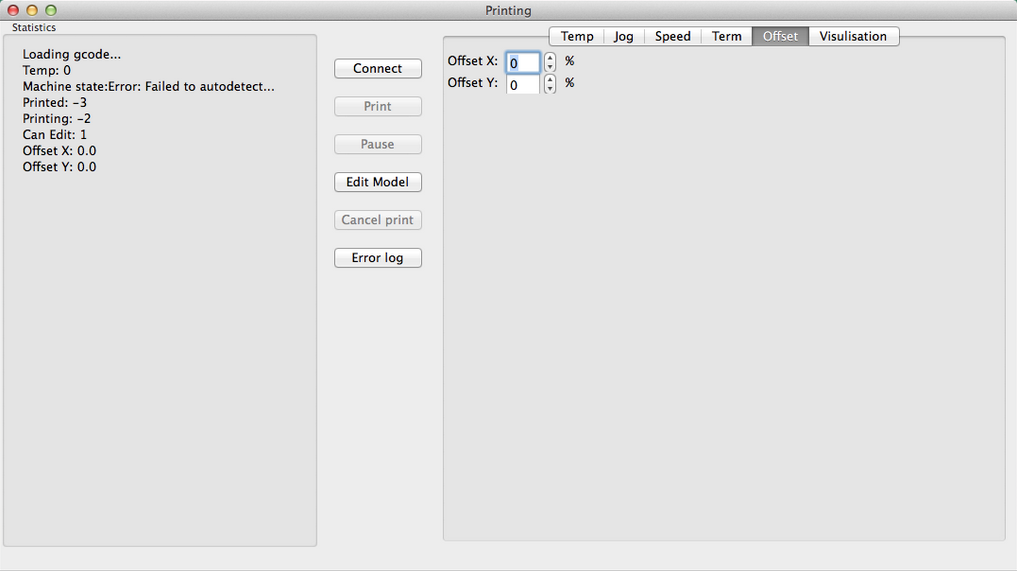
\includegraphics[width=4in]{CuraCustomTab.png}
  \caption{Cura print window showing new custom tab.}
  \label{figure:CuraCustomTab}
\end{figure}

In this tab we added the ability to shift a given print layer by specified amounts in the X and Y axes. The way this works is by replacing the X and Y parameter values with new numbers. The offsetting amount can be specified in the user interface. Using regular expressions we insured the line was a G1 instruction, then scanned it for the X and Y parameters which we extracted. We then modified these values and replaced the \verb|X<number> Y<number>| component of the line.

This operation is already of immediate utility to the end user. A common error scenario, shown below, is that the nozzle is jogged by an external source or problem with the rubber belts or stepper motors, making the print offset by a certain amount. If the user can simply jog the printed model back by the opposite amount in our user interface, this error can be mitigated.

\begin{figure}[H]
  \centering
  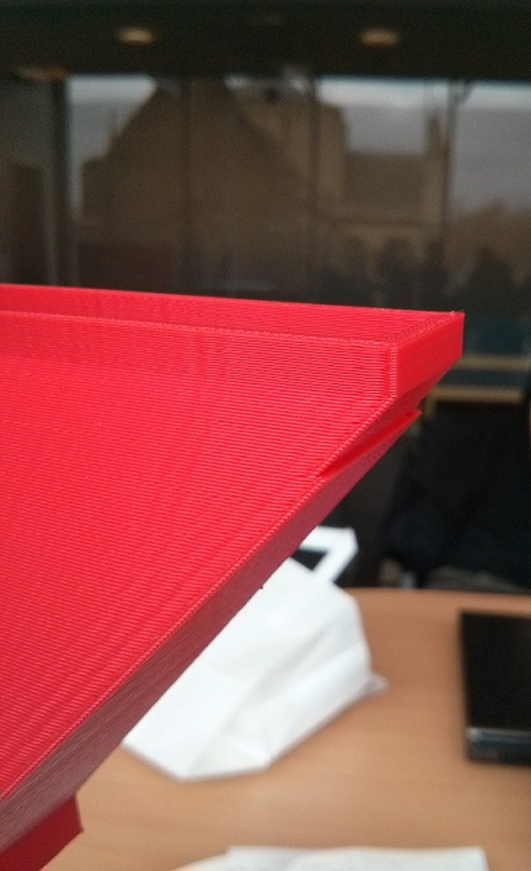
\includegraphics[height=4in]{FoggerOffset.png}
  \caption{Photograph of the scenario described here that can be solved by our offsetting feature.}
  \label{figure:FoggerOffset}
\end{figure}

This is one example of a manipulation but once this was possible it opened the door to more advanced just-in-time control, such as the full range of affine transformations of translation, scaling, reflection, rotation and shearing. These operations come with the limitation that they can currently only be performed globally on one whole slice at a time. There may be an additional need to inspect the command history for the more complex transformations.




\section{Improved Duration Estimation}
	With the ability to take control of and manipulate the list of commands sent to the 3D printer, we next wanted to tackle constructing a basic model of the printer in software.

	Or goal was to estimate the time that it takes to print a given line of g-code with a high degree of accuracy, in order to estimate the total time for an entire print. The reason we wished to implement this feature is that the leading two 3D printer software packages, MakerWare for MakerBot and Cura for Ultimaker have very poor accuracy, coarse estimate times for the 3D prints. Having the ability to predict printing times more accurately is a desirable feature for the end user.

	The first step in performing this task was to look at any speed indicators in the g-code. We found that any movement command followed by an F parameter set the speed of the printer. For example, we might see:
\begin{verbatim}
G1 X100 Y100 F1000
\end{verbatim}

In accordance with the specifications~\ref{reference:47} the printer should obey the F parameters. Next we needed to work out the units used. To test this we crafted some custom g-code files which performed very controlled simple shapes (single-lines up to ten zig-zags) without any rafts or other more complex structure material commands. This showed how many lines the printer should execute and, allowing for easy timing. We only performed X and Y (horizontal) motion as we assumed (correctly, as we shall see later) that the printer mechanism for horizontal and vertical motion occurs at a different speed.

	Using a stopwatch, we timed a complete print from the first motion of the print head. We used the lap function of the stopwatch to lap the initial part of the print at the point the head finished its move from the starting location to the centre of the base plate. This allowed us later to subtract this time from our measurement.

	Using the ten zig-zag code and keeping other print settings constant we varied the F number inside the g-code file and took a number of measurements. We came to the conclusion that the units of F were in millimeters per second. Next, we needed to measure the speed of the Z (vertical) motion. We constructed a new set of g-code files to raise the printhead 50 layers (one layer is one physical level on the Z axis). We varied only the F number. Our measurements were as follows in Table~\ref{table:speedTimes}.

\begin{table}[h]{\begin{minipage}{\textwidth}
\begin{tabular}{| l || l | l | l | l | l | l | l |}
\hline
Speed in g-code: & F16000 & F8000 & F4000 & F2000 & F1000 & F500 & F250 \\\hline
50 Z lines (seconds): & 5.20 & 5.30 & 5.00 & 5.20 & 6.68 & 6.55 & 12.36 \\\hline
Effective speed (mm/min): & 577 & 577 & 600 & 577 & 449 & 458 & 243 \\\hline

\end{tabular}
\caption{Printer Z speed estimation time trials.}
\label{table:speedTimes}
\end{minipage} }
\end{table}

Our conclusion was that the vertical speed could not go faster than approximately 600 mm/min. What this means for F values lower than 2000 was unreliable as an estimator. To simplify the situation we used the results above as an F-value-to-speed mapping in our code.

Now that we had the speed units for both horizontal and vertical motion, we could use some regular expressions to extract the coordinates of the print head at a given point in time from successive pairs of g-code commands and calculate the distances between them. We now had enough information to estimate the duration of any particular motion using Figure~\ref{figure:TDS}.

\begin{figure}[H]
  \centering
  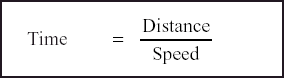
\includegraphics[width=3in]{TDS.png}
  \caption{\ref{reference:49}}
  \label{figure:TDS}
\end{figure}

By totalling up the estimated durations for each of the lines of g-code in our file we can produce an overall estimate of the print time. We then pre-computed the durations of prints from the raw g-code and compared them to the duration of a print of that file. We found that the error was approximately 10\%, with more errors the larger the print. From this we deduced that there is more at play than the X, Y and Z motions of the motors.

Some possibilities are that the motors have an additional delay when turning corners, accelerating up from a stopped state and decelerating down to stop. We weren't able to spot these extra times as our timing method (stopwatch and visual inspection) is not sufficiently precise and a different physical measurement system would need to be developed.

While they would require further refinement to be commercially interesting as a virtual (software) printer model, the calculation we provide is still a significant improvement on estimates provided in the commercial software. Regardless, we now have the ability to provide a rough but still strongly improved duration estimate of a print.





\section{Parameter Adjustments}
\label{section:ParameterAdjustments}
Previous sections have shown that we can inspect, manipulate and perform calculations of the g-code when it is close to being printed. We also extended Cura's graphical user interface to allow the end user to manipulate the print just-in-time with a delay of as little as one layer.
	With error mitigation in mind, we looked at the properties of the printed object itself, to see whether we could apply the technique of manipulating the g-code to improve the print quality and reduce errors. This was a natural progression from our initial gains, which allowed us to diversify further and manipulate the print parameters to be adjusted mid-print.
Some useful changes now possible were: thickening the walls of the object, or increasing the internal plastic fill structure. This capability is useful as large or particularly low sloping walls are prone to sagging due to the difficulty in supporting themselves in extreme situations (such as when they are too far removed from the available underlying support). In contrast, reducing the wall thickness or fill density, can prove equally useful, when for example material is running too low to complete a print job or upon realising that a print would take too long otherwise.
The image below shows examples of the initial combination of X/Y shifts made possible along with some more advanced transformations that demonstrate parameter adjustments such as global scaling up, scaling down and changes in the amount of internal fill.

\begin{figure}[H]
  \centering
  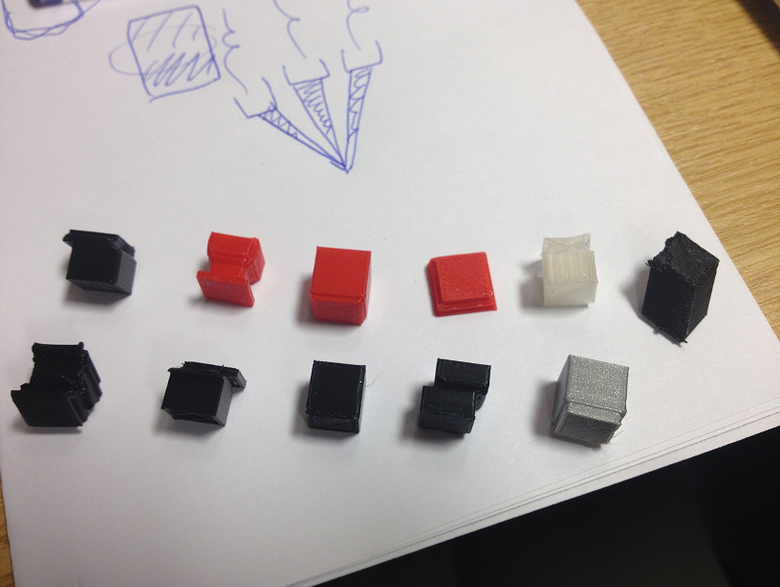
\includegraphics[width=4in]{RedWhiteSilver.png}
  \caption{Black printed cubes show original X/Y shifting ability. Red, white and silver cubes show more advanced global scaling and fill changes.}
  \label{figure:RedWhiteSilver}
\end{figure}

The global properties of the model such as fill density could previously only be set up at the beginning of the print using the preset function in the Cura software, locking in the user's decisions once the print has begun. Below is our extended list of possible changes now available after starting a print, in Figure~\ref{figure:CuraScalingRobot}.

\begin{figure}[H]
  \centering
  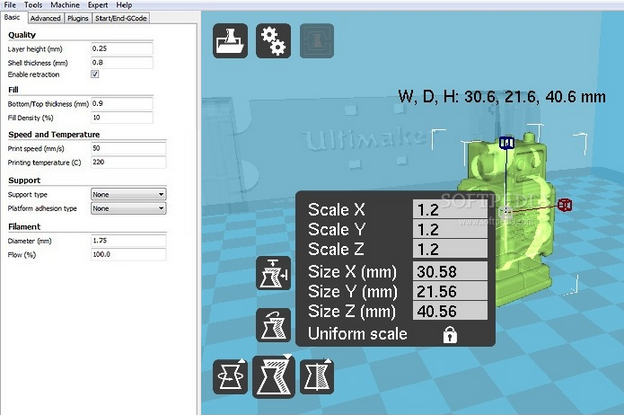
\includegraphics[width=4in]{CuraScalingRobot.png}
  \caption{Cura print properties window and scaling user interface.}
  \label{figure:CuraScalingRobot}
\end{figure}

Now follows a summary of extractable information about the printer in Table~\ref{table:CuraProperties}
\begin{table}[h]{\begin{minipage}{\textwidth}
\begin{tabular}{| p{3cm} | p{2cm} | p{8.5cm} |}
\hline

Property name & Units & Purpose\\\hline
Layer height & mm & The vertical thickness of one layer of plastic, used to determine the total height of the print. This is determined by the thickness set by the physical constraints of the printer nozzle.\\\hline
Shell thickness & mm & The horizontal thickness of the object wall --- the millimetre size, which is a multiple of the plastic thickness and is converted into the number of walls needed to be printed to accomplish the desired shell thickness.\\\hline
Enable retraction & True/False & Allow the printer to retract the filament between movements where no printing should be done --- to prevent webbing of loose filament.\\\hline
Bottom/top thickness & mm & The vertical thickness of the bottom and top caps of the object.\\\hline
Fill density & \% & The percentage of the internal space of the object that should be filled with supporting plastic. If this percentage is less than 100\% and more than 0\% the inside is filled with a regular cross-hatching pattern, otherwise at 0\% is empty and 100\% is solid.\\\hline
Print speed & mm/s & The baseline speed of the printer head, not taking into account the acceleration and layer changes.\\\hline
Printing temperature & \degree{}C & The temperature at which the printer is manually set to extrude plastic, normally 230\degree{}C for ABS~\ref{reference:50}. A heating element in the printer will automatically adjust to reach the correct temperature before enabling the print button on Cura and then self regulate throughout.\\\hline
Support type & Multiple values & Additional support structures may be printed in anticipation of overhanging parts. This setting determines whether or not to do so and the type of support to use.\\\hline
Platform adhesion type & Multiple values & Whether or not to print additional layers underneath the object to improve adhesion to the print bed (to avoid shifting or warping during the print). This can be a raft (a rough but more adhesive layer of plastic) or a brim (additional wall support underneath where the shell will lie).\\\hline
Diameter & mm & The diameter of the filament --- this should be set to the value specified by the filament manufacturer.\\\hline
Flow & \% & Flow rate of extruded filament --- 100\% is normal, unimpeded flow.\\\hline

\end{tabular}
\caption{A summary of extractable information about an object from Cura.}
\label{table:CuraProperties}
\end{minipage} }
\end{table}

	Of these printer properties we found that the fill density and scale/rotation properties were the most immediately useful for error mitigation. Fill density reduction is useful if a user is running out of filament and doesn't wish the print to fail halfway through, therefore preferring for the print to finish with with less internal fill than originally intended. Scaling is also useful for this scenario as it reduces the object size to use less filament. Scaling and rotation are also an example of printer property of particular interest to those using 3D printing as a design tool or for creative experiments. 

	As mentioned, we wanted to be able to make changes whilst the printing is taking place and apply changes to the pending layers. This required the introduction of a new algorithm:

\begin{description}
\item[1. Regenerate the original file] Take the original file, reset its print properties to include the newly specified properties and reslice it. This operation is performed by the CuraEngine component each time behind the scenes whenever a property is changed.
\item[2. Align the new line to the currently printing line] Looking in the newly generated model, find the line that corresponds to the line in the original file already printing. This is done by recording the layer index at the time of the resend operation and using this to index into the new file. Since all manipulations are performed at layer boundaries, this indexing process will correctly locate the g-code line to resume from in the new file.
\item[3. Splice the two files together at the indexed line] Replace future lines in the g-code list with the lines from the new file, starting at the line found in step 2.
\item[4. Send future lines to the printer from the new spliced file] This will happen automatically using our newly implemented Cura buffer which we created to send lines layer by layer.
\end{description}

	We then introduced a new button to the Cura interface that allows us to commit the modifications made by the user. An existing Cura button design was used for the button and it can be found to the right of the print button in the new interface as shown in Figure~\ref{figure:NewButton}.

\begin{figure}[H]
  \centering
  
\includegraphics[width=1.5cm]{NewButton.png}
  \caption{New `resend' button.}
  \label{figure:NewButton}
\end{figure}

There are no restrictions on how the set parameters can be changed in the user interface, meaning that in addition to gradual changes in the infill, rotations and scaling, the user can change other parameters specified in the Cura interface, or change them by larger amounts than expected. While this is true in principle and works for the initial more simple changes to the object being printed, more extreme changes encounter difficulties. For example Figure~\ref{figure:MissingLayers} shows problems arising when fill density was increased or reduced very sharply.

\begin{figure}[H]
  \centering
  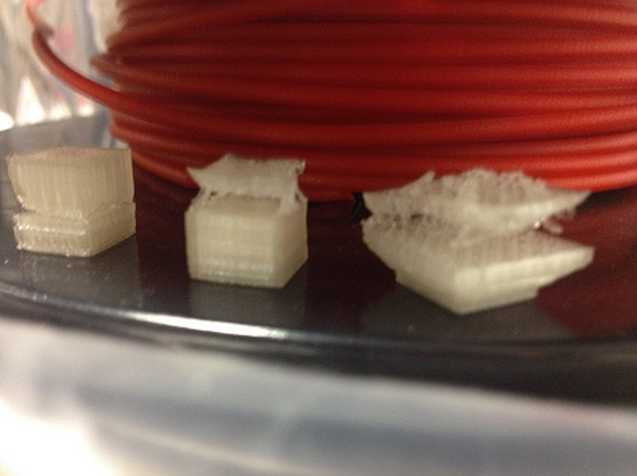
\includegraphics[width=4in]{MissingLayers.png}
  \caption{Changing the fill percentage too drastically means the new fill layer will not stick onto the previous layer, leaving large vertical gaps in the cubes here.}
  \label{figure:MissingLayers}
\end{figure}

While the parameter adjustments are useful and functional, they need to be used with the caveat that they are unrestricted and require expertise, with care when for example applied for error mitigation purposes.






\section{Adaptive Skirt}
\label{section:AdaptiveSkirt}
\subsubsection{What is a skirt?}
\begin{figure}[H]
  \centering
  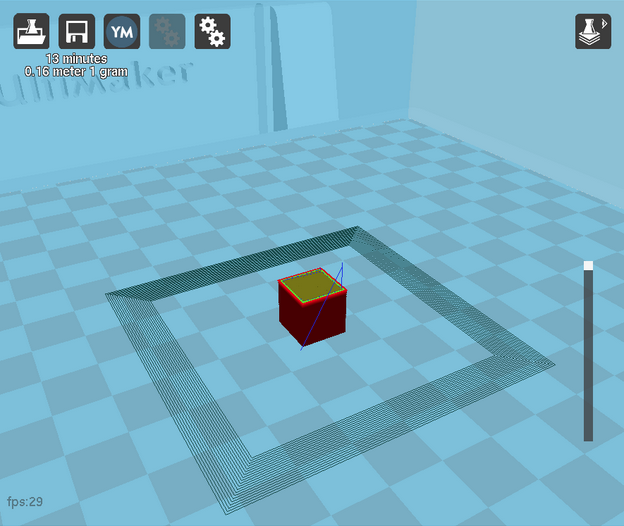
\includegraphics[width=4in]{WhatIsASkirt.png}
  \caption{Image of large skirt in Cura. The skirt is the series of dark squares surrounding the red cube.}
  \label{figure:WhatIsASkirt}
\end{figure}

One of the limitations of FDM 3D printers is that there are often problems with them not extruding plastic. There are many reasons for this including: problems with the motor, running out of filament or the nozzle being blocked. The problem is particularly prevalent at the start of a print when it needs to heat up. It often takes a while for it to begin extruding, meaning that the first layer will not be printed, resulting in a failed print.

In an attempt to solve this, Cura gives the user the option to add a preparation step called a skirt. A skirt will print a perimeter around the outside of where the object will be printed of a thickness set by the user. The purpose of this stage is to give the printer more time to begin extruding before it actually starts printing the object.

\subsubsection{Problems with existing skirt}
The skirt is a good idea, however, it doesn't completely solve the problem. Sometimes even with a skirt the printer doesn't extrude. We observed that there are two common reasons for this: 

The printer needs even more time for filament to heat or to be pushed up to the nozzle
The nozzle is blocked and no matter the skirt settings it will not extrude 

These problems are then routinely solved by straightforward steps:

Increasing the size of the skirt --- giving the printer more time to start extruding
Increasing the temperature of the nozzle and extrusion amount to clear blockage

While these solutions are quite straight forward they aren't perfect. Printing a large skirt is a poor use of time and resources, however it is the tradeoff to the risk of wasted time restarting a print that failed to extrude because of a small skirt. Additionally heating the nozzle and increasing the extrusion amount is a very manual process. You need to stop the print, increase the temperature, then manually turn the motor to clear the blockage. In our implementation of the skirt we wanted to automate these processes.

\subsubsection{Our implementation}
We allow the user to set the parameters of the print, such as the size of the skirt, as usual, however, we encourage users to make the skirt as large as possible. Once the CuraEngine slices the model into g-code we perform some additional steps. 

Firstly in the g-code generated we find the temperature value chosen for the print. This is in a g-code command, M109, which sets the temperature to a specified value then waits for the temperature to reach this value before executing the next command. We replace the chosen temperature of the M109 command with 250 degrees, then add an additional command M104 with the original temperature. M104 is also a temperature command, however it doesn't require for the printer to wait before executing the next command. This means that the temperature is at 250 degrees when it starts printing but slowly cools down as the skirt is printed. 

As the skirt is very large we wanted a way to be able to stop the skirt and begin printing the object once the printer was extruding successfully. As we already implemented the buffer and layer-based control but couldn't use the switching g-code file method from the previous section we needed to come up with a new solution. This was to create two versions of the cumulative histogram and g-code list; one with the skirt, one without. Then at a time specified by the user switch between the two. 

Creating the cumulative histogram and g-code list including the skirt followed the original method discussed in Section~\ref{section:BufferControl} with one adaption. As the skirt is actually a very large layer due to the encouraged large size and we only have layer-based control to alter g-code we needed to create additional `fake-layers'. Each of these fake layers comprise one subsection of the larger skirt layer, effectively dividing it into a more easily interruptible set of subtasks.This means that after a number of skirt g-code commands are added to the g-code list, we create a layer that doesn't really exist but allows us to effectively switch g-code at in between layers. As skirts can be different shapes we needed to dynamically set the number of skirt commands that should be in a `fake-layer'. We found that one fifth of the number of layers to be a good threshold. 

The skirtless g-code list and cumulative histogram was slightly more complex. We again made use of the commands in the g-code to know what part of the g-code we were in and when new layers needed to be added. When in the skirt section, marked with a comment, we didn't add any of the commands to the g-code list. However, as we have layer-based control we needed to have a matching number of layers as the previous cumulative histogram. So, `fake-layers' were also added to this cumulative histogram and g-code list with a single null g-code command, which, is never sent to the firmware. This allows us to make use of the existing switching g-code system. 

We then updated the GUI to have a button that allows the user to switch the g-code once the skirt was successfully being printed. Originally we allowed this to be done at any time, however, we quickly noticed that if the temperature was still very high then each of the layers didn't adhere to each other very well. As a result we only allow the user to switch the g-code once the temperature has reached the original value. If the user never presses the button to switch the g-code then the complete skirt will print before printing the object.




\section{Geometry Manipulation}
\label{section:GeometryManipulation}
\begin{figure}[H]
  \centering
  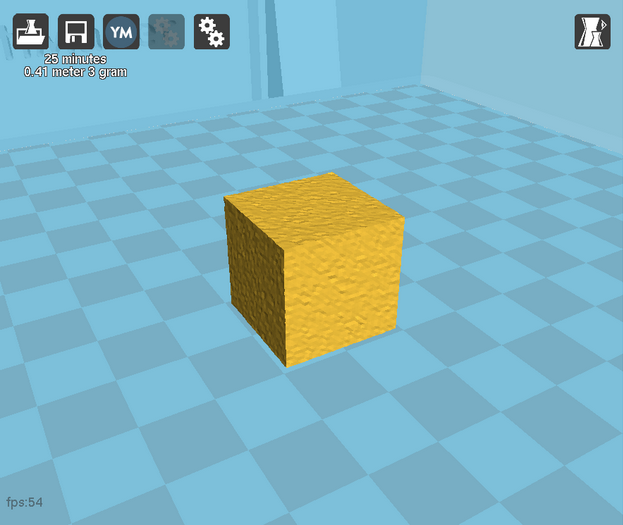
\includegraphics[width=4in]{CubeNoise.png}
  \caption{Example of cube with noise applied.}
  \label{figure:CubeNoise}
\end{figure}

In the previous sections we have demonstrated two methods to alter the g-code during a print. Neither of the methods change the geometry of the object being printed. In this section we show that our system offers the potential to alter the geometry of the object while printing. While we have achieved a proof of concept, further development would be required to constitute a complete use case. 

In the pre-existing Cura source code, when a 3D model is loaded the file is read and stored in a basic data structure that only contains information about the vertices of the mesh, i.e., as a point cloud. At this time the data structure holds no information about how the vertices connect to one another. Without the connectivity information it is difficult to perform meaningful deformation operations on the mesh, however we can perturb each vertex individually. Figure~\ref{figure:CubeNoise} demonstrates how each vertex can have additive zero-mean white noise applied to it. This proof of concept tool is available to the user through an extra button that has been added to the scene view of Cura that will add the random white noise to each of the vertices, re-slice the edited model and update the rendered version of the object. If happy with the change, the user can use the re-send button, discussed in Section~\ref{section:ParameterAdjustments}, to send the updated g-code to the firmware from the next layer.


\chapter{Evaluation}
\section{Case Studies}
To evaluate our project we have selected a number of use cases that show a significant improvement from the results previously possible. The three use cases are: the adaptive skirt, preventing holes in the top of objects and fixing misaligned objects. Each of these make use of the custom buffer system we implemented.

\subsection{Adaptive Skirt}
The adaptive skirt outlined in Section~\ref{section:AdaptiveSkirt} allows the user to print a large skirt for the model, with the added feature that they can stop printing the skirt and begin printing the model at a time of their choice. The aim of the adaptive skirt is to save time lost on restarting prints and clearing blockages, as well as make better use of material. Many of the survey respondents stipulated that they incur these errors on a regular basis~\ref{section:AppendixA}.

For this case study we attempted to print a simple 1 x 1 x 1 cm cube using the original and new systems.  

\subsubsection{Original Cura implementation}
Our first attempt to print the cube using the original Cura implementation used the smallest skirt available to the user (size 1), meaning only one outline around the cube was printed. The print head didn't begin extruding until well into the first layer of the actual cube. When the printer began extruding it didn't stick to the bed, turning into a ball of mess, seen in Figure~\ref{figure:SkirtOld1}.

\begin{figure}[H]
  \centering
  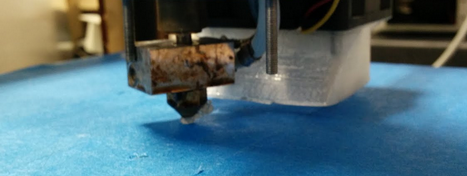
\includegraphics[width=4in]{SkirtOld1.png}
  \caption{First failure using original Cura.}
  \label{figure:SkirtOld1}
\end{figure}

In the final attempt to print the cube the skirt was set to size 20, which was a success and can be seen in Figure~\ref{figure:SkirtOld2}. The print was successful, however in comparison to the pre-set skirt of size 1 it wasted material. 

\begin{figure}[H]
  \centering
  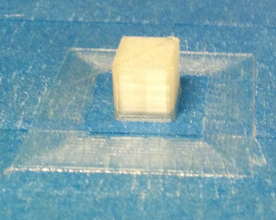
\includegraphics[width=4in]{SkirtOld2.png}
  \caption{Success using original Cura.}
  \label{figure:SkirtOld2}
\end{figure}

\subsubsection{Our implementation}
Using our adaptive skirt the print only took one attempt. We selected a skirt of size 20 but manually switched the g-code to the skirtless version after 5 outlines were printed successfully, Figure~\ref{figure:SkirtNew1}. This was a significant time saving as it avoided restarting prints. It's worth noting that during the case study there were no nozzle blockages, which would have made getting a successful print with the original implementation even more time consuming. Our custom skirt is preset to begin at size 20 to allow time for the nozzle to un-block if necessary.


\begin{figure}[H]
  \centering
  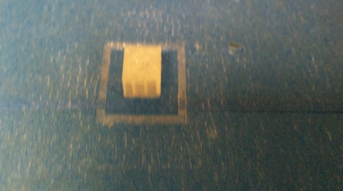
\includegraphics[width=4in]{SkirtNew1.png}
  \caption{Success using our adaptive skirt.}
  \label{figure:SkirtNew1}
\end{figure}

\subsection{Holes In Top Of Object}
The second case study makes use of the parameter adjustment technique outlined in Section~\ref{section:ParameterAdjustments}. We tackle the problem of when hollow objects develop holes in the top. These holes are indeterministic and are caused when the first of the top layers have nothing underneath as support

For this case study we use a truncated upside down pyramid, with the following parameters: uniform scale of 4.0, no infill, a layer height of 0.1mm, wall thickness of 0.3 and top/bottom thickness of 0.6. 

\subsubsection{Original Cura implementation}

For the original implementation we had two unsuccessful prints due to problems with the printer not extruding before the model printed successfully. No parameters were changed during the print and the result can be seen in Figure~\ref{figure:PyramidOld1}. The image shows that the thickness of the top is uneven with holes in it. We consider this a failed print. This is a mild example of holes appearing in objects, if the model were scaled up it would likely have many more and larger holes. 

\begin{figure}[H]
  \centering
  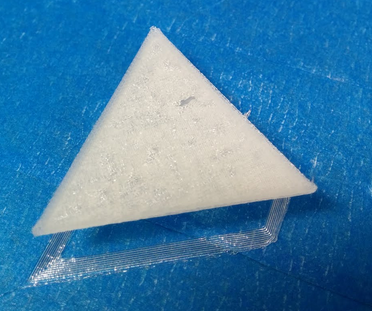
\includegraphics[width=4in]{PyramidOld1.png}
  \caption{Example hole in top of model.}
  \label{figure:PyramidOld1}
\end{figure}

\subsubsection{Our implementation}
We printed the same truncated pyramid using our implementation. After three of the six layers were printed it was evident from visual observation that holes would appear. We were able to change some parameters just-in-time to solve the problem. We performed a non-uniform scale along the Z-axis to 4.5 (as opposed to the pre-set scale of 4.0), stretching the model, then increasing the bottom/top thickness to 1.2 (which as the bottom was already printed was applied to the failing top only). This prevented any holes in the top of the model, however, it did leave an artefact on the profile of the model, which can be seen in Figure~\ref{figure:PyramidNew1}. In some cases this could be an acceptable artefact but not it others. This technique of only scaling in the Z axis would also work well for rectangular shapes but for this specific geometry it doesn't.

In a second attempt to solve the problem after three of the six top layers of the original model were printed the parameters were changed, this time with a uniform scale of 4.5 and a top/bottom thickness of 1.2. This resulted in an object (Figure~\ref{figure:PyramidNew2}) with no holes but was slightly larger than the original model.

\begin{figure}[H]
  \centering
  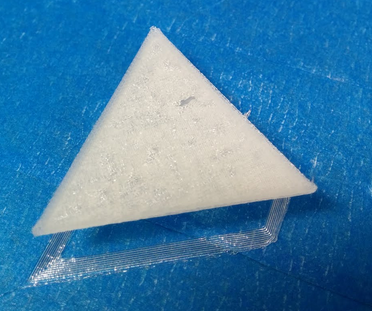
\includegraphics[width=4in]{PyramidOld1.png}
  \caption{Limitation scaling in only Z axis.}
  \label{figure:PyramidNew1}
\end{figure}

\begin{figure}[H]
  \centering
  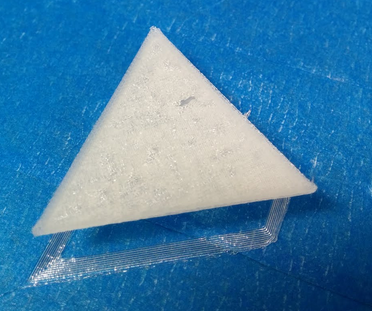
\includegraphics[width=4in]{PyramidOld1.png}
  \caption{Our final result.}
  \label{figure:PyramidNew2}
\end{figure}

In this case study we demonstrated that we can prevent holes in the top of models by changing the parameters mid-print. We are unable to do this without leaving an artefact and it will depend on the purpose of the model what artefacts the user is willing to accept. Those survey respondents working in commercial 3d printing for example are likely to have higher standards for object finish, however many stipulated that they currently perform hand finishing to models. This would be possible given our suggested solutions, see Section~\ref{section:AppendixA}.

\begin{figure}[H]
  \centering
  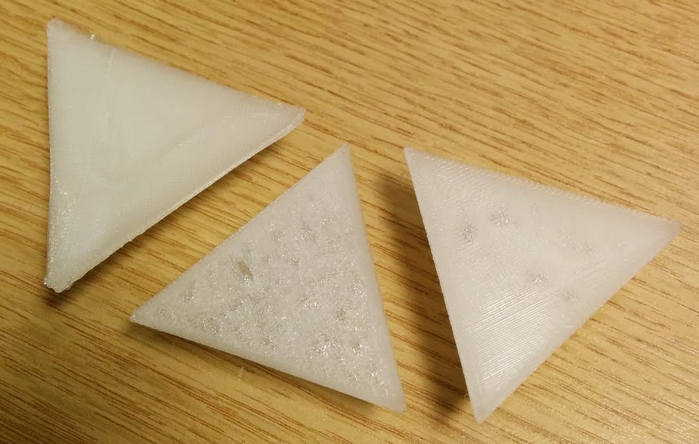
\includegraphics[width=4in]{PyramidsAll.png}
  \caption{The three models printed for this case study.}
  \label{figure:PyramidsAll}
\end{figure}

\subsection{Layer Misalignment}
The final case study we used to evaluate our system is the example of layer misalignment. This problem occurs when a printer is jogged or when the belts that moving the print head slip. One of our commercial survey respondents reported that misalignment is a problem that has cost him customers in the past, when prints fail due to this reason and delivery times are pushed back as a result, see Section~\ref{section:AppendixA}.

We printed a 3 x 3 x 3 cube with infill of 20\% and manually caused it to be offset by a constant value.

\subsubsection{Original Cura implementation}
Using the original Cura we printed the object with the manual offset, which can be seen in Figure~\ref{figure:Misalign1}. This is a completely failed print as there is no possible way to solve the error. 

\begin{figure}[H]
  \centering
  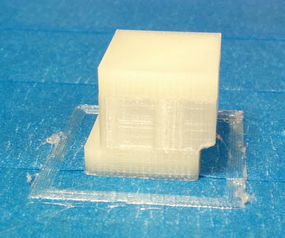
\includegraphics[width=4in]{Misalign1.png}
  \caption{Example of failed print due to layer misalignment.}
  \label{figure:Misalign1}
\end{figure}

\subsubsection{Our implementation}
Using our implementation we offset the cube but then use the parameter adjustment to realign the cube and continue printing. We made two attempts of this, which can been seen in Figures~\ref{figure:Misalign2}~and~\ref{figure:Misalign3}.

\begin{figure}[H]
  \centering
  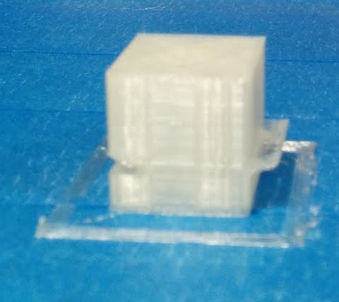
\includegraphics[width=4in]{Misalign2.png}
  \caption{First example of correcting misalignment.}
  \label{figure:Misalign2}
\end{figure}

\begin{figure}[H]
  \centering
  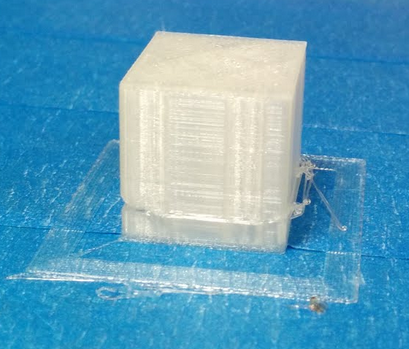
\includegraphics[width=4in]{Misalign3.png}
  \caption{Second attempt for correcting misalignment.}
  \label{figure:Misalign3}
\end{figure}

In the first example it took 4 layers from when the offset occurred to correct the alignment. This results in there being a very noticeable ledge sticking out from the cube and missing chunk on the opposite side. The second attempt only took 2 layers so both of the artefacts are much smaller. It is possible to manually sand down the ledge sticking out, however, the missing chunk will always be visible. 

This second attempt is a significant improvement on the previous outcome of an unusable print. The biggest challenge is for the user knowing how far exactly the model has become misaligned. A problem we propose a solution for in the future work section.   


\section{Overview}
In our three case studies we have demonstrated a number of techniques to mitigate common errors encountered when 3D printing.  Some of the techniques come with tradeoffs that will always be specific to the object being printed and the user will need to decide what artefacts are acceptable or not. As a result of these artefacts our future work outlines some potential ways to reduce them.  




\chapter{Future Work}
\section{Improved Geometry Manipulation}
We first introduced Geometry Manipulation in Section~\ref{section:GeometryManipulation} with a proof-of-concept example of applying noise to the model. As the pre-existing Cura implementation stores the model as a point cloud that contains no edge information, it was difficult to manipulate the geometry of the object meaningfully. 

Subsequently, the first area of future work would be to store the vertex connectivity information in a half-edge data structure. A half-edge data structure would provide additional information about the shape of the model, allowing for efficient (in terms of both computation and memory) processing of a mesh and further, would more useful geometry manipulation algorithms~\ref{reference:51}.

A possible application to investigate would be using the laplace-beltrami operator, to deform the shape of the model to mitigate errors. Concretely, if a model with a large overhang was beginning to sag, you could smoothly deform the mesh and in doing so, counteract the sag and ensure it remained balanced, most importantly allowing the shape to remain similar to the original. This approach would need to take into consideration that the printed and committed layers cannot move. 




\section{Automated Error Mitigation}
The error mitigation applications enabled by our system outlined in Section~\ref{section:Method} requires the user to interact with the software for the errors to be avoided. This is in itself very useful, however, it requires the user to be somewhat experienced with 3D printing. For example, to use the translation application outlined in Sections~\ref{section:GCodeManipulation}~and~\ref{section:ParameterAdjustments} to correct for a print, which has become misaligned, the user needs to know exactly how far the print has translated --- a nontrivial task. Similarly, for a user to make use of the custom skirt feature, they must be familiar with the type of texture and thickness that the filament should be before switching to print the object. From our personal experience as we performed these tasks more and more, they become simple and repetitive. 

As a result, an area for future research is automating this process so that no human interaction is required to mitigate errors. An automation process like this would require a computer vision system to monitor the printer in real-time, recording what is physically being printed. As this imaging data is fed back in real-time (algorithms that would need to be developed) could compare the input data with the g-code to ensure that there are no errors. If an error is detected, such as the object becoming misaligned, then the system would need to decide which one of a series of preprogrammed but parameterised operations, in this case translation, needed to be performed. The system would also have to determine the parameters of those operations, such as their direction and distance. 

The automated system has many facets and challenges. Firstly as the filament being printed is very thin, it could prove to be a challenge to accurately record what is being printed. A potential option would be to use a calibrated thermal camera, as this would provide more accurate information to confirm that the printer is extruding successfully. Once the data is accurately recorded it then needs to be compared to the original g-code. Perhaps this could be done using a homography to map the data to a plane, reducing the problem to comparing each layer as it is printed to the corresponding layer of g-code in 2D. The final and perhaps hardest challenge, would be once a misalignment is identified calculating what operation and its parameters needed to be performed. We can see that there is much potential for automating the processes we have developed with the use of additional sensing equipment and image processing techniques. We hope that our work has opened up this new research avenue of automated systems and made it more feasible to enter.




\section{Design Tool}
3D printing is strongly associated with creative, artistic design processes, it is often used in rapid prototyping processes, utilised for example by designers and artists who wish to produce initial models of their work to gain quick feedback during the design process~\ref{reference:53},~\ref{reference:55},~\ref{reference:56}.

	Just-in-time control gives a greater degree of interaction with an object, not possible before. Achieving control of the printer just-in-time has opened out many different potential applications, the group spent some time considering the opportunity of how this control might be used to enhance the creative design process. To begin this investigation we conducted a semi structured interview with the artist Tom Lomax who designs using software packages such as Rhino and produces work on 3D printers. Tom has his own SLS printer and also sends models away to commercial print companies~\ref{reference:52}. 

\begin{figure}[H]
  \centering
  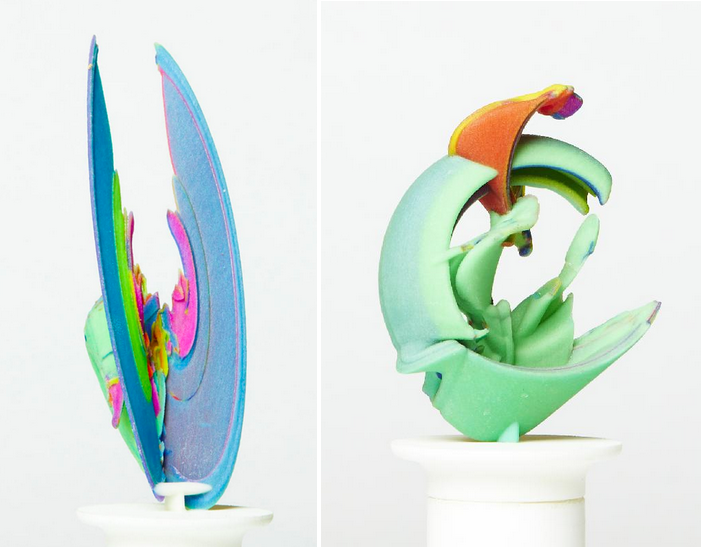
\includegraphics[width=4in]{Lomax.png}
  \caption{\textit{Raphael} and \textit{Caffiel} created by Tom Lomax, printed on an SLS machine.}
  \label{figure:Lomax}
\end{figure}

From this discussion it became apparent that enabling control after the print process opens an entirely new kind of design interaction into the creative process, giving artists the opportunity to use the physical object as a continuous source upon which to make spontaneous decisions, having them enacted in the moment of realisation. 

	Input during the print of 3D objects was previously limited to a number of key points in time involving: 
\begin{enumerate}
\item Computer based design: Interfacing with computer software packages such as Rhino
\item Post print: Affixing material to the object post-print, altering the colour and finish of the surfaces
\end{enumerate}

	The level of input that the artist can have during the creative process is thus restricted by the technology. This is not a chosen restriction but an imposed one, yet the techniques of Rapid prototyping and its associated 3D print processes have been added to the education curriculum of established fine arts programs in which such processes are strongly affiliated with artistic genres of sculpture and collage~\ref{reference:54},~\ref{reference:70}. This shows that design and creativity are being shaped by the kinds of technology and associated processes available 

	Collage, perhaps less well known than sculpture, means `to paste' in French and first emerged as a fine art when cubists Pablo Picasso and George Braque incorporated pasted papers and objects into their designs~\ref{reference:58}. Using software packages such as OpenSCAD (more often associated with engineering design) artists can configure collage designs, visualising components as a single sculpture and editing them as they are being printed to create novel configurations. One can imagine how as a piece is altered as it is being printed the artist or designer can determine the initial shape of congruent pieces yet to be printed and carry out similar deformations to build in an organic way that is informed by visual feedback of the physical object.

	In order to enrich the artist's impact on their work, the group discussed possibilities of adding elaborate control systems. For example creating a haptic pottery wheel and affixing it to the 3D printer that the user could sculpt upon, sending information to the printer to change the object being printed according to the hand sculpted model and creating an interactive design experience. This idea applies to other design processes than fine art, for example the architect Frank Gehry uses sculpted prototypes in order to work out the final shape of his building designs, as with the Guggenheim Bilbao~\ref{reference:57}, Figure~\ref{figure:GuggenheimBilbao}.

\begin{figure}[H]
  \centering
  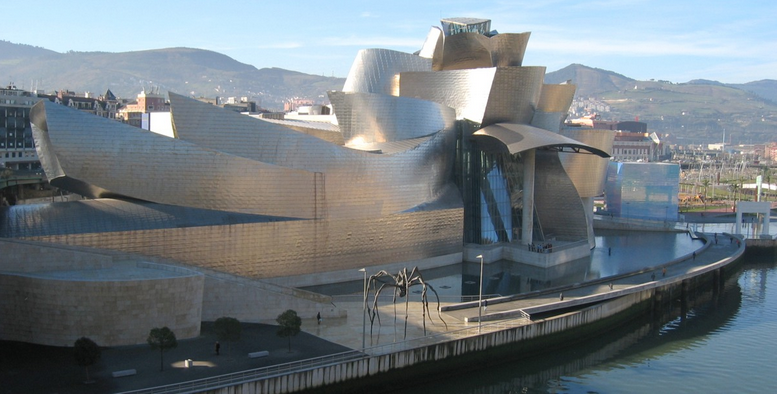
\includegraphics[width=4in]{GuggenheimBilbao.png}
  \caption{Guggenheim Bilbao.}
  \label{figure:GuggenheimBilbao}
\end{figure}

Having a physical 3D print out would enable the geometries to be tested in real time and demonstrated in a 3D printed prototype as the designer allows their sculpted object to evolve using visual feedback that they are acquainted with. 

	Another idea that the group considered was to use a holographic representation of the object being printed, to communicate with the user about potential ways that the shape of the object might be changed next, given the existing geometries of the already printed sections. This idea of calculating and adjusting the shape geometries is similar to the research mentioned in Section~\ref{section:CurrentApproaches}, such as Make it Stand.

	A finished product that is fitted with a haptic device would allow the 3D print process to become intertwined with the design phase, altering the design object as it is being printed. The end product might be used primarily by artists and novice 3D print users looking to experiment with novel processes.   



\chapter{Conclusion}
Our project began with a proposal to advance 3D printing by adding real-time control and exploring potential applications. We collaborated as an interdisciplinary team to research the state-of-the-art of 3D printing. We built upon this by developing a number of novel applications to assist in reducing the of errors incurred during 3D printing. 

In the early stages of our project we realised that achieving real-time control of the printer would be too challenging for an initial goal. So we began focusing on achieving just-in-time control of the printer and the potential applications. We found there to be two distinct categories: error mitigation and design tools. We chose to focus on the former as from first hand experience we knew of the frustrations of failed 3D prints.   

In our prior art research we found that much of the literature around reducing print errors was a pre-processing step to ensure that the geometry was optimised for successful printing. We were interested in changing the model being printed as it was being printed, which we used to make the novel contribution of a responsive error mitigation system. 

As part of our preliminary research we investigated how the existing 3D print system worked, focusing on the open-source application Cura. As a result we developed an extension of Cura with a number of adaptations. Central to these was a buffer control system that controls what g-code and when it is sent to the printer. Introducing this buffer control system allowed us to develop a number of novel error mitigation applications. One of the applications is a way to adjust print parameters such as fill density, then produce new g-code, which is switched for the old g-code at the next available layer. This allows the user to fix many problems. A common problem (the most common problem that we encountered) is printhead misalignment. Another new application was the introduction of a custom skirt that preempts common problems encountered when a print has newly started. We achieved this by adjusting the temperature and increasing the extrusion amount before an object is printed. Once the printer is ready to begin printing the model the user can choose when to start doing so. 

We evaluated our project through a number of surveys, gathering quantitative and qualitative information for 3D printer users. It was clear from the evaluation that 3D printing remains error prone and our extension of Cura solved some of these issues successfully.  

Finally we outlined a number of areas of future work. These were automating the error mitigation examples that we have designed and are currently manual. Automation would reduce the error rate further and make 3D printing more accessible. The second area of future research is into how our just-in-time control could be applied into novel interfaces to improve the design process.





\chapter{Appendix}
\label{section:AppendixA}
https://github.com/JWHennessey/Cura

% Bibliography
\nocite{*}
\bibliographystyle{plain}
\bibliography{bibliography}

\end{document}
